% Options for packages loaded elsewhere
\PassOptionsToPackage{unicode}{hyperref}
\PassOptionsToPackage{hyphens}{url}
\PassOptionsToPackage{dvipsnames,svgnames,x11names}{xcolor}
%
\documentclass[
  letterpaper,
  DIV=11,
  numbers=noendperiod]{scrartcl}

\usepackage{amsmath,amssymb}
\usepackage{iftex}
\ifPDFTeX
  \usepackage[T1]{fontenc}
  \usepackage[utf8]{inputenc}
  \usepackage{textcomp} % provide euro and other symbols
\else % if luatex or xetex
  \usepackage{unicode-math}
  \defaultfontfeatures{Scale=MatchLowercase}
  \defaultfontfeatures[\rmfamily]{Ligatures=TeX,Scale=1}
\fi
\usepackage{lmodern}
\ifPDFTeX\else  
    % xetex/luatex font selection
\fi
% Use upquote if available, for straight quotes in verbatim environments
\IfFileExists{upquote.sty}{\usepackage{upquote}}{}
\IfFileExists{microtype.sty}{% use microtype if available
  \usepackage[]{microtype}
  \UseMicrotypeSet[protrusion]{basicmath} % disable protrusion for tt fonts
}{}
\makeatletter
\@ifundefined{KOMAClassName}{% if non-KOMA class
  \IfFileExists{parskip.sty}{%
    \usepackage{parskip}
  }{% else
    \setlength{\parindent}{0pt}
    \setlength{\parskip}{6pt plus 2pt minus 1pt}}
}{% if KOMA class
  \KOMAoptions{parskip=half}}
\makeatother
\usepackage{xcolor}
\usepackage[left=0.3in, right=0.3in, top=0.3in, bottom=0.3in]{geometry}
\setlength{\emergencystretch}{3em} % prevent overfull lines
\setcounter{secnumdepth}{-\maxdimen} % remove section numbering
% Make \paragraph and \subparagraph free-standing
\makeatletter
\ifx\paragraph\undefined\else
  \let\oldparagraph\paragraph
  \renewcommand{\paragraph}{
    \@ifstar
      \xxxParagraphStar
      \xxxParagraphNoStar
  }
  \newcommand{\xxxParagraphStar}[1]{\oldparagraph*{#1}\mbox{}}
  \newcommand{\xxxParagraphNoStar}[1]{\oldparagraph{#1}\mbox{}}
\fi
\ifx\subparagraph\undefined\else
  \let\oldsubparagraph\subparagraph
  \renewcommand{\subparagraph}{
    \@ifstar
      \xxxSubParagraphStar
      \xxxSubParagraphNoStar
  }
  \newcommand{\xxxSubParagraphStar}[1]{\oldsubparagraph*{#1}\mbox{}}
  \newcommand{\xxxSubParagraphNoStar}[1]{\oldsubparagraph{#1}\mbox{}}
\fi
\makeatother

\usepackage{color}
\usepackage{fancyvrb}
\newcommand{\VerbBar}{|}
\newcommand{\VERB}{\Verb[commandchars=\\\{\}]}
\DefineVerbatimEnvironment{Highlighting}{Verbatim}{commandchars=\\\{\}}
% Add ',fontsize=\small' for more characters per line
\usepackage{framed}
\definecolor{shadecolor}{RGB}{241,243,245}
\newenvironment{Shaded}{\begin{snugshade}}{\end{snugshade}}
\newcommand{\AlertTok}[1]{\textcolor[rgb]{0.68,0.00,0.00}{#1}}
\newcommand{\AnnotationTok}[1]{\textcolor[rgb]{0.37,0.37,0.37}{#1}}
\newcommand{\AttributeTok}[1]{\textcolor[rgb]{0.40,0.45,0.13}{#1}}
\newcommand{\BaseNTok}[1]{\textcolor[rgb]{0.68,0.00,0.00}{#1}}
\newcommand{\BuiltInTok}[1]{\textcolor[rgb]{0.00,0.23,0.31}{#1}}
\newcommand{\CharTok}[1]{\textcolor[rgb]{0.13,0.47,0.30}{#1}}
\newcommand{\CommentTok}[1]{\textcolor[rgb]{0.37,0.37,0.37}{#1}}
\newcommand{\CommentVarTok}[1]{\textcolor[rgb]{0.37,0.37,0.37}{\textit{#1}}}
\newcommand{\ConstantTok}[1]{\textcolor[rgb]{0.56,0.35,0.01}{#1}}
\newcommand{\ControlFlowTok}[1]{\textcolor[rgb]{0.00,0.23,0.31}{\textbf{#1}}}
\newcommand{\DataTypeTok}[1]{\textcolor[rgb]{0.68,0.00,0.00}{#1}}
\newcommand{\DecValTok}[1]{\textcolor[rgb]{0.68,0.00,0.00}{#1}}
\newcommand{\DocumentationTok}[1]{\textcolor[rgb]{0.37,0.37,0.37}{\textit{#1}}}
\newcommand{\ErrorTok}[1]{\textcolor[rgb]{0.68,0.00,0.00}{#1}}
\newcommand{\ExtensionTok}[1]{\textcolor[rgb]{0.00,0.23,0.31}{#1}}
\newcommand{\FloatTok}[1]{\textcolor[rgb]{0.68,0.00,0.00}{#1}}
\newcommand{\FunctionTok}[1]{\textcolor[rgb]{0.28,0.35,0.67}{#1}}
\newcommand{\ImportTok}[1]{\textcolor[rgb]{0.00,0.46,0.62}{#1}}
\newcommand{\InformationTok}[1]{\textcolor[rgb]{0.37,0.37,0.37}{#1}}
\newcommand{\KeywordTok}[1]{\textcolor[rgb]{0.00,0.23,0.31}{\textbf{#1}}}
\newcommand{\NormalTok}[1]{\textcolor[rgb]{0.00,0.23,0.31}{#1}}
\newcommand{\OperatorTok}[1]{\textcolor[rgb]{0.37,0.37,0.37}{#1}}
\newcommand{\OtherTok}[1]{\textcolor[rgb]{0.00,0.23,0.31}{#1}}
\newcommand{\PreprocessorTok}[1]{\textcolor[rgb]{0.68,0.00,0.00}{#1}}
\newcommand{\RegionMarkerTok}[1]{\textcolor[rgb]{0.00,0.23,0.31}{#1}}
\newcommand{\SpecialCharTok}[1]{\textcolor[rgb]{0.37,0.37,0.37}{#1}}
\newcommand{\SpecialStringTok}[1]{\textcolor[rgb]{0.13,0.47,0.30}{#1}}
\newcommand{\StringTok}[1]{\textcolor[rgb]{0.13,0.47,0.30}{#1}}
\newcommand{\VariableTok}[1]{\textcolor[rgb]{0.07,0.07,0.07}{#1}}
\newcommand{\VerbatimStringTok}[1]{\textcolor[rgb]{0.13,0.47,0.30}{#1}}
\newcommand{\WarningTok}[1]{\textcolor[rgb]{0.37,0.37,0.37}{\textit{#1}}}

\providecommand{\tightlist}{%
  \setlength{\itemsep}{0pt}\setlength{\parskip}{0pt}}\usepackage{longtable,booktabs,array}
\usepackage{calc} % for calculating minipage widths
% Correct order of tables after \paragraph or \subparagraph
\usepackage{etoolbox}
\makeatletter
\patchcmd\longtable{\par}{\if@noskipsec\mbox{}\fi\par}{}{}
\makeatother
% Allow footnotes in longtable head/foot
\IfFileExists{footnotehyper.sty}{\usepackage{footnotehyper}}{\usepackage{footnote}}
\makesavenoteenv{longtable}
\usepackage{graphicx}
\makeatletter
\newsavebox\pandoc@box
\newcommand*\pandocbounded[1]{% scales image to fit in text height/width
  \sbox\pandoc@box{#1}%
  \Gscale@div\@tempa{\textheight}{\dimexpr\ht\pandoc@box+\dp\pandoc@box\relax}%
  \Gscale@div\@tempb{\linewidth}{\wd\pandoc@box}%
  \ifdim\@tempb\p@<\@tempa\p@\let\@tempa\@tempb\fi% select the smaller of both
  \ifdim\@tempa\p@<\p@\scalebox{\@tempa}{\usebox\pandoc@box}%
  \else\usebox{\pandoc@box}%
  \fi%
}
% Set default figure placement to htbp
\def\fps@figure{htbp}
\makeatother

\usepackage{fvextra}
\DefineVerbatimEnvironment{Highlighting}{Verbatim}{breaklines,commandchars=\\\{\}}
\DefineVerbatimEnvironment{OutputCode}{Verbatim}{breaklines,commandchars=\\\{\}}
\KOMAoption{captions}{tableheading}
\makeatletter
\@ifpackageloaded{caption}{}{\usepackage{caption}}
\AtBeginDocument{%
\ifdefined\contentsname
  \renewcommand*\contentsname{Table of contents}
\else
  \newcommand\contentsname{Table of contents}
\fi
\ifdefined\listfigurename
  \renewcommand*\listfigurename{List of Figures}
\else
  \newcommand\listfigurename{List of Figures}
\fi
\ifdefined\listtablename
  \renewcommand*\listtablename{List of Tables}
\else
  \newcommand\listtablename{List of Tables}
\fi
\ifdefined\figurename
  \renewcommand*\figurename{Figure}
\else
  \newcommand\figurename{Figure}
\fi
\ifdefined\tablename
  \renewcommand*\tablename{Table}
\else
  \newcommand\tablename{Table}
\fi
}
\@ifpackageloaded{float}{}{\usepackage{float}}
\floatstyle{ruled}
\@ifundefined{c@chapter}{\newfloat{codelisting}{h}{lop}}{\newfloat{codelisting}{h}{lop}[chapter]}
\floatname{codelisting}{Listing}
\newcommand*\listoflistings{\listof{codelisting}{List of Listings}}
\makeatother
\makeatletter
\makeatother
\makeatletter
\@ifpackageloaded{caption}{}{\usepackage{caption}}
\@ifpackageloaded{subcaption}{}{\usepackage{subcaption}}
\makeatother

\usepackage{bookmark}

\IfFileExists{xurl.sty}{\usepackage{xurl}}{} % add URL line breaks if available
\urlstyle{same} % disable monospaced font for URLs
\hypersetup{
  pdftitle={Stats 102B HW 4},
  pdfauthor={Bryan Mui - UID 506021334},
  colorlinks=true,
  linkcolor={blue},
  filecolor={Maroon},
  citecolor={Blue},
  urlcolor={Blue},
  pdfcreator={LaTeX via pandoc}}


\title{Stats 102B HW 4}
\author{Bryan Mui - UID 506021334}
\date{}

\begin{document}
\maketitle


Due Wed, June 4, 11:00 pm

\begin{Shaded}
\begin{Highlighting}[]
\FunctionTok{library}\NormalTok{(tidyverse)}
\end{Highlighting}
\end{Shaded}

\begin{verbatim}
-- Attaching core tidyverse packages ------------------------ tidyverse 2.0.0 --
v dplyr     1.1.4     v readr     2.1.5
v forcats   1.0.0     v stringr   1.5.1
v ggplot2   3.5.2     v tibble    3.2.1
v lubridate 1.9.4     v tidyr     1.3.1
v purrr     1.0.4     
-- Conflicts ------------------------------------------ tidyverse_conflicts() --
x dplyr::filter() masks stats::filter()
x dplyr::lag()    masks stats::lag()
i Use the conflicted package (<http://conflicted.r-lib.org/>) to force all conflicts to become errors
\end{verbatim}

\begin{Shaded}
\begin{Highlighting}[]
\NormalTok{train }\OtherTok{\textless{}{-}} \FunctionTok{read\_csv}\NormalTok{(}\StringTok{"train\_data.csv"}\NormalTok{)}
\end{Highlighting}
\end{Shaded}

\begin{verbatim}
Rows: 600 Columns: 601
-- Column specification --------------------------------------------------------
Delimiter: ","
dbl (601): X1, X2, X3, X4, X5, X6, X7, X8, X9, X10, X11, X12, X13, X14, X15,...

i Use `spec()` to retrieve the full column specification for this data.
i Specify the column types or set `show_col_types = FALSE` to quiet this message.
\end{verbatim}

\begin{Shaded}
\begin{Highlighting}[]
\NormalTok{val }\OtherTok{\textless{}{-}} \FunctionTok{read\_csv}\NormalTok{(}\StringTok{"validation\_data.csv"}\NormalTok{)}
\end{Highlighting}
\end{Shaded}

\begin{verbatim}
Rows: 200 Columns: 601
-- Column specification --------------------------------------------------------
Delimiter: ","
dbl (601): X1, X2, X3, X4, X5, X6, X7, X8, X9, X10, X11, X12, X13, X14, X15,...

i Use `spec()` to retrieve the full column specification for this data.
i Specify the column types or set `show_col_types = FALSE` to quiet this message.
\end{verbatim}

\newpage

\subsection{Problem 1}\label{problem-1}

Consider the function

\[
f(x) = \frac{1}{4} x^4 - x^2 + 2x
\]

\subsubsection{\texorpdfstring{Part
\((\alpha)\)}{Part (\textbackslash alpha)}}\label{part-alpha}

Using the pure version of Newton's algorithm report \(x_k\) for
\(k = 20\) (after running the algorithm for 20 iterations) based on the
following 5 initial points:

\begin{enumerate}
\def\labelenumi{\arabic{enumi}.}
\tightlist
\item
  \(x_0 = −1\)
\item
  \(x_0 = 0\)
\item
  \(x_0 = 0.1\)
\item
  \(x_0 = 1\)
\item
  \(x_0 = 2\)
\end{enumerate}

\textbf{Newton's pure algorithm is as follows:}

\begin{enumerate}
\def\labelenumi{\arabic{enumi}.}
\tightlist
\item
  Select \(x_0 \in \mathbb{R}^n\)
\item
  While stopping criterion \textgreater{} tolerance do:

  \begin{enumerate}
  \def\labelenumii{\arabic{enumii}.}
  \tightlist
  \item
    \(x_{k+1} = x_k - [\nabla^2f(x_k)]^{-1} \nabla f(x_k)\)
  \item
    Calculate value of stopping
    criterion(\(|f(x_{k+1}) - f(x_k)| \leq \epsilon\))
  \end{enumerate}
\end{enumerate}

Gradient:
\(\nabla f(x) = \frac{\partial}{\partial x} = f'(x) = x^3 - 2x + 2\)

Hessian:
\(\nabla^2 f(x) = \frac{\partial^2}{\partial x^2} = f''(x) = 3x^2 - 2\)

\begin{Shaded}
\begin{Highlighting}[]
\CommentTok{\# params}
\NormalTok{max\_iter }\OtherTok{\textless{}{-}} \DecValTok{20}
\NormalTok{starting\_points }\OtherTok{\textless{}{-}} \FunctionTok{c}\NormalTok{(}\SpecialCharTok{{-}}\DecValTok{1}\NormalTok{, }\DecValTok{0}\NormalTok{, }\FloatTok{0.1}\NormalTok{, }\DecValTok{1}\NormalTok{, }\DecValTok{2}\NormalTok{)}
\NormalTok{stopping\_tol }\OtherTok{\textless{}{-}} \FloatTok{1e{-}6}


\CommentTok{\# algorithm}
\NormalTok{newton\_pure\_alg }\OtherTok{\textless{}{-}} \ControlFlowTok{function}\NormalTok{(max\_iter, starting\_point, stopping\_tol) \{}
\NormalTok{  beta }\OtherTok{\textless{}{-}}\NormalTok{ starting\_point}
\NormalTok{  iterations\_ran }\OtherTok{\textless{}{-}} \DecValTok{0}
\NormalTok{  betas\_vec }\OtherTok{\textless{}{-}} \FunctionTok{c}\NormalTok{(beta)}
  
\NormalTok{  obj }\OtherTok{\textless{}{-}} \ControlFlowTok{function}\NormalTok{(x) \{}
  \FunctionTok{return}\NormalTok{(}\DecValTok{1}\SpecialCharTok{/}\DecValTok{4} \SpecialCharTok{*}\NormalTok{ x}\SpecialCharTok{\^{}}\DecValTok{4} \SpecialCharTok{{-}}\NormalTok{ x}\SpecialCharTok{\^{}}\DecValTok{2} \SpecialCharTok{+} \DecValTok{2}\SpecialCharTok{*}\NormalTok{x)}
\NormalTok{  \}}
\NormalTok{  grad }\OtherTok{\textless{}{-}} \ControlFlowTok{function}\NormalTok{(x) \{}
\NormalTok{    x}\SpecialCharTok{\^{}}\DecValTok{3} \SpecialCharTok{{-}} \DecValTok{2}\SpecialCharTok{*}\NormalTok{x }\SpecialCharTok{+} \DecValTok{2}
\NormalTok{  \}}
\NormalTok{  hessian }\OtherTok{\textless{}{-}} \ControlFlowTok{function}\NormalTok{(x) \{}
    \DecValTok{3}\SpecialCharTok{*}\NormalTok{x}\SpecialCharTok{\^{}}\DecValTok{2} \SpecialCharTok{{-}} \DecValTok{2}
\NormalTok{  \}}
  
  \ControlFlowTok{for}\NormalTok{(i }\ControlFlowTok{in} \DecValTok{1}\SpecialCharTok{:}\NormalTok{max\_iter) \{}
\NormalTok{    beta\_new }\OtherTok{\textless{}{-}}\NormalTok{ beta }\SpecialCharTok{{-}}\NormalTok{ (}\FunctionTok{grad}\NormalTok{(beta) }\SpecialCharTok{/} \FunctionTok{hessian}\NormalTok{(beta))}
\NormalTok{    betas\_vec[i}\SpecialCharTok{+}\DecValTok{1}\NormalTok{] }\OtherTok{\textless{}{-}}\NormalTok{ beta\_new}
    \ControlFlowTok{if}\NormalTok{(}\FunctionTok{abs}\NormalTok{(beta\_new }\SpecialCharTok{{-}}\NormalTok{ beta) }\SpecialCharTok{\textless{}=}\NormalTok{ stopping\_tol) \{ }\ControlFlowTok{break}\NormalTok{ \}}
\NormalTok{    beta }\OtherTok{\textless{}{-}}\NormalTok{ beta\_new}
\NormalTok{  \}}
\NormalTok{  iterations\_ran }\OtherTok{\textless{}{-}}\NormalTok{ i}
  \FunctionTok{return}\NormalTok{(}\FunctionTok{list}\NormalTok{(}\AttributeTok{iterations=}\NormalTok{iterations\_ran, }\AttributeTok{betas=}\NormalTok{betas\_vec))}
\NormalTok{\}}

\CommentTok{\# running the alg}
\FunctionTok{cat}\NormalTok{(}\StringTok{"Newton\textquotesingle{}s Algorithm(Pure) For Different Starting Points: }\SpecialCharTok{\textbackslash{}n}\StringTok{"}\NormalTok{)}
\end{Highlighting}
\end{Shaded}

\begin{verbatim}
Newton's Algorithm(Pure) For Different Starting Points: 
\end{verbatim}

\begin{Shaded}
\begin{Highlighting}[]
\ControlFlowTok{for}\NormalTok{ (starting\_point }\ControlFlowTok{in}\NormalTok{ starting\_points) \{}
\NormalTok{  result }\OtherTok{\textless{}{-}} \FunctionTok{newton\_pure\_alg}\NormalTok{(max\_iter, starting\_point, stopping\_tol)}
  \FunctionTok{cat}\NormalTok{(}\StringTok{"}\SpecialCharTok{\textbackslash{}n}\StringTok{Starting Point:"}\NormalTok{, starting\_point, }\StringTok{"}\SpecialCharTok{\textbackslash{}n}\StringTok{Iterations:"}\NormalTok{, result}\SpecialCharTok{$}\NormalTok{iterations, }\StringTok{"}\SpecialCharTok{\textbackslash{}n}\StringTok{Betas:}\SpecialCharTok{\textbackslash{}n}\StringTok{"}\NormalTok{)}
  \FunctionTok{print}\NormalTok{(result}\SpecialCharTok{$}\NormalTok{betas)}
  \FunctionTok{cat}\NormalTok{(}\StringTok{"}\SpecialCharTok{\textbackslash{}n}\StringTok{"}\NormalTok{, }\StringTok{"\textasciitilde{}\textasciitilde{}\textasciitilde{}\textasciitilde{}\textasciitilde{}\textasciitilde{}\textasciitilde{}\textasciitilde{}\textasciitilde{}\textasciitilde{}\textasciitilde{}\textasciitilde{}\textasciitilde{}\textasciitilde{}\textasciitilde{}\textasciitilde{}\textasciitilde{}\textasciitilde{}\textasciitilde{}\textasciitilde{}\textasciitilde{}\textasciitilde{}\textasciitilde{}\textasciitilde{}\textasciitilde{}\textasciitilde{}\textasciitilde{}\textasciitilde{}\textasciitilde{}\textasciitilde{}\textasciitilde{}\textasciitilde{}\textasciitilde{}\textasciitilde{}\textasciitilde{}\textasciitilde{}\textasciitilde{}\textasciitilde{}\textasciitilde{}\textasciitilde{}\textasciitilde{}\textasciitilde{}\textasciitilde{}\textasciitilde{}\textasciitilde{}\textasciitilde{}\textasciitilde{}\textasciitilde{}\textasciitilde{}\textasciitilde{}\textasciitilde{}\textasciitilde{}\textasciitilde{}\textasciitilde{}\textasciitilde{}"}\NormalTok{, }\StringTok{"}\SpecialCharTok{\textbackslash{}n}\StringTok{"}\NormalTok{)}
\NormalTok{\}}
\end{Highlighting}
\end{Shaded}

\begin{verbatim}

Starting Point: -1 
Iterations: 8 
Betas:
[1] -1.000000 -4.000000 -2.826087 -2.146719 -1.842326 -1.772848 -1.769301
[8] -1.769292 -1.769292

 ~~~~~~~~~~~~~~~~~~~~~~~~~~~~~~~~~~~~~~~~~~~~~~~~~~~~~~~ 

Starting Point: 0 
Iterations: 20 
Betas:
 [1] 0 1 0 1 0 1 0 1 0 1 0 1 0 1 0 1 0 1 0 1 0

 ~~~~~~~~~~~~~~~~~~~~~~~~~~~~~~~~~~~~~~~~~~~~~~~~~~~~~~~ 

Starting Point: 0.1 
Iterations: 20 
Betas:
 [1] 1.000000e-01 1.014213e+00 7.965577e-02 1.009099e+00 5.222653e-02
 [6] 1.003965e+00 2.332944e-02 1.000804e+00 4.806795e-03 1.000035e+00
[11] 2.072525e-04 1.000000e+00 3.865288e-07 1.000000e+00 1.345590e-12
[16] 1.000000e+00 0.000000e+00 1.000000e+00 0.000000e+00 1.000000e+00
[21] 0.000000e+00

 ~~~~~~~~~~~~~~~~~~~~~~~~~~~~~~~~~~~~~~~~~~~~~~~~~~~~~~~ 

Starting Point: 1 
Iterations: 20 
Betas:
 [1] 1 0 1 0 1 0 1 0 1 0 1 0 1 0 1 0 1 0 1 0 1

 ~~~~~~~~~~~~~~~~~~~~~~~~~~~~~~~~~~~~~~~~~~~~~~~~~~~~~~~ 

Starting Point: 2 
Iterations: 9 
Betas:
 [1]  2.0000000  1.4000000  0.8989691 -1.2887793 -2.1057673 -1.8292000
 [7] -1.7717158 -1.7692966 -1.7692924 -1.7692924

 ~~~~~~~~~~~~~~~~~~~~~~~~~~~~~~~~~~~~~~~~~~~~~~~~~~~~~~~ 
\end{verbatim}

\subsubsection{Part (i) What do you
observe?}\label{part-i-what-do-you-observe}

\begin{figure}[H]

{\centering \pandocbounded{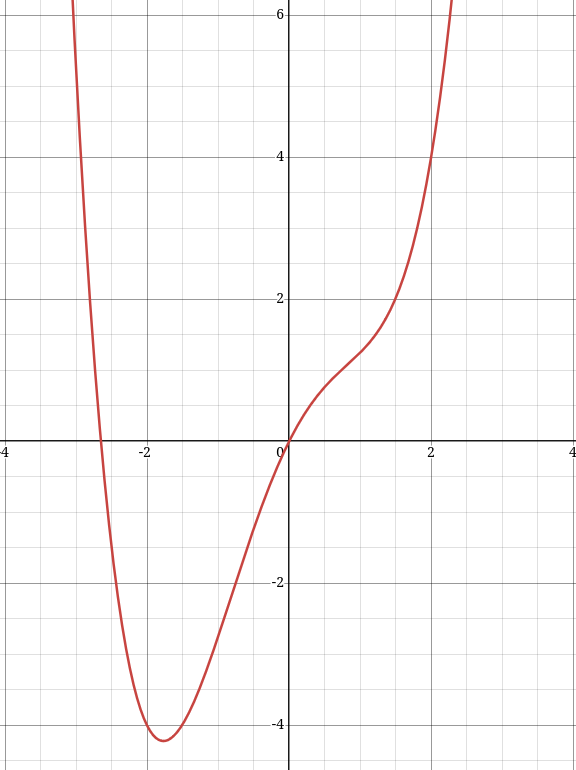
\includegraphics[keepaspectratio]{images/clipboard-3935267595.png}}

}

\caption{Plot of the Objective Function f(x)}

\end{figure}%

I observe that given the code output, the algorithms that did not
converge oscillate between 0 1 0 1, which means that it gets stuck when
the curvature of the graph changes. I think that the graph goes from
concave up to concave down at this point, which will mess up the
gradient descent calculation. The Hessian is the second derivative, or
second order gradient, meaning the concavity of the function will affect
the sign. Given the update step,
\(x_{k+1} = x_k - [\nabla^2f(x_k)]^{-1} \nabla f(x_k)\), we can see that
if the Hessian's sign goes from negative to positive(concave down to
concave up) or vice versa then it will change the sign of the update
step to be gradient ascent(away from the minimum) rather than towards it

\subsubsection{Part (ii) How can you fix the issue reported in
(i)?}\label{part-ii-how-can-you-fix-the-issue-reported-in-i}

I believe that the issue is normally fixed by drawing the graph and
getting and understanding of the shape, and therefore choosing one of
the starting points that does end up converging. However, in cases where
that isn't possible(if the function cannot be plotted or is very
complex), I would try to build a vector of possible starting points and
perform a grid search where we run the algorithm on multiple starting
points and various parameters. This would allow us to find a starting
point where the algorithm would converge. From the lecture slides, there
are alternative Newton's algorithms like Newton's algorithm with
damping, which I would implement if there is too much trouble with the
pure Newton's algorithm.

\newpage

\subsection{Problem 2}\label{problem-2}

Consider the data in the train data.csv file. The first 600 columns
correspond to the predictors and the last column to the response y.

\subsubsection{Part (i) Implement that proximal gradient algorithm for
Lasso regression, by modifying appropriately your code from Homework
1.}\label{part-i-implement-that-proximal-gradient-algorithm-for-lasso-regression-by-modifying-appropriately-your-code-from-homework-1.}

To select a good value for the regularization parameter \(λ\) use the
data in the validation data.csv to calculate the sum-of-squares error
validation loss.

The Proximal Gradient Descent Algorithm(LASSO):

\subsubsection{\texorpdfstring{Part(ii) Show a plot of the training and
validation loss as a function of iterations. Report the number of
regression coefficients estimated as zero based on the best value of
\(λ\) you
selected.}{Part(ii) Show a plot of the training and validation loss as a function of iterations. Report the number of regression coefficients estimated as zero based on the best value of λ you selected.}}\label{partii-show-a-plot-of-the-training-and-validation-loss-as-a-function-of-iterations.-report-the-number-of-regression-coefficients-estimated-as-zero-based-on-the-best-value-of-ux3bb-you-selected.}

Plotting Training Loss:

Plotting Validation Loss:




\end{document}
